\documentclass[11pt, oneside]{article}  
% \documentclass[fleqn,10pt]{wlpeerj}


\usepackage{geometry}  
%\usepackage{nunito}
\usepackage{cmbright}
\geometry{letterpaper}   
\usepackage{cite}
\usepackage{graphicx}				% Use pdf, png, jpg, or eps§ with pdflatex; use eps in DVI mode
								% TeX will automatically convert eps --> pdf in pdflatex	
\usepackage{tcolorbox}
\usepackage{amssymb}
\usepackage{longtable}
\usepackage{amsmath}
\usepackage{booktabs}
% \usepackage{emoji}
\usepackage{url}
\usepackage{color}
\definecolor{c1}{rgb}{0.12, 0.56, 1.0}
%SetFonts
\usepackage{xspace}
\usepackage{xcolor}
\usepackage{caption}
\usepackage{subcaption}
\usepackage{authblk} 

\usepackage{sectsty} 
\definecolor{cool_blue}{RGB}{24, 132, 193}
\sectionfont{\color{c1}\selectfont}
\subsectionfont{\color{c1}\selectfont}
\subsubsectionfont{\color{c1}\selectfont}
% \paragraphfont{\color{gray}\selectfont}
\subparagraphfont{\color{gray}\selectfont}

\definecolor{fruitpushorange}{RGB}{255, 127, 0}
\newcommand{\data}{$(s_1, ..., s_k)$\xspace}

\usepackage{soul}
\DeclareRobustCommand{\cms}[1]{ {\begingroup\sethlcolor{fruitpushorange}\hl{(cms:) #1}\endgroup} }
%SetFonts

\sloppy 

\title{Bi-objective ant colony optimization of the risky, robot-team orienteering problem}
\author[1]{Cory M. Simon}
\author[2]{Jeffrey Richley}
\author[2]{Lucas Overbey}
\author[2]{Darleen Perez-Lavin}
\affil[1]{School of Chemical, Biological, and Environmental Engineering. Oregon State University. Corvallis, OR. USA.}
% \affil[]{\texttt{cory.simon@oregonstate.edu}}
\affil[2]{Naval Information Warfare Center Atlantic. Charleston, SC. USA.}
% \corrauthor[1]{Cory M. Simon}{cory.simon@oregonstate.edu}

% \keywords{Keyword1, Keyword2, Keyword3}



%\flushbottom
% \maketitle
%\thispagestyle{empty}


%\affil[*]{}
% \date{}							% Activate to display a given date or no date

\begin{document}
\maketitle

\begin{abstract}
In many applications e.g., resource delivery, patrolling, and information-gathering, a team of mobile [aerial, ground, or aquatic] robots must coordinate their trails in some environment to cooperatively achieve some team-level objective. Robots may risk failure/destruction while traversing some environments, owing to dangerous conditions or the presence of adversaries capable of attacking them. Then, robot trail-planning should account for these risks.

Herein, we use ant colony optimization to find the [approximate] Pareto-optimal set of robot trail plans for the bi-objective, risky team orienteering problem, where (i) a team of robots are mobile within an environment abstracted as a graph (nodes: locations, edges: paths between locations); (ii) each node offers a reward to the team when visited by a robot; (iii) the traversal of each edge imposes a risk of robot failure/destruction; and (iv) the two [often, competing] team objectives are to maximize the expected (a) team reward and (b) number of robots that survive the mission. 
Presenting the Pareto-optimal set of robot trail plans to the downstream decision-maker allows them to choose the plans that balance, according to their values, the two objectives. As a case study, we illustrate with an information-gathering mission in a nuclear power plant from a Defense Advanced Research Projects Agency (DARPA) robots challenge.
\end{abstract}

\clearpage


\section{Introduction}
\subsection{Applications of a team of mobile robots}
Mobile [aerial, ground, or aquatic] robots equipped with sensors, actuators, and/or cargo have applications in agriculture (eg. planting and harvesting crops, spraying pesticide, monitoring crop health) \cite{santos2020path}, commerce (eg.\ order fulfillment in warehouses) \cite{wurman2008coordinating}, the delivery of goods \cite{coelho2014thirty}, search-and-rescue \cite{queralta2020collaborative}, chemical, biological, radiological, or nuclear incident response (eg.\ safely localizing the source(s) and assessing the severity of the incident) \cite{murphy2012projected}, environmental monitoring \cite{dunbabin2012robots}, safety monitoring of an industrial chemical plant  \cite{soldan2014towards}, forest fire monitoring and fighting \cite{merino2012unmanned}, and military surveillance and reconnaissance. 

Deploying a \emph{team} of robots for a mission, as opposed to a single robot, can increase spatial coverage, decrease the time to achieve the objectives, and allow for resilience if a robot fails.

We often for a team of mobile robots to coordinate their paths in the environment to cooperatively achieve a shared, team-level objective \cite{parker2007distributed,lesser1999cooperative}.
For example, consider the team orienteering problem (TOP) \cite{gunawan2016orienteering,vansteenwegen2011orienteering}. 
The environment, in which a team of robots can traverse, is abstracted as a graph (nodes: locations; edges: spatial connections between locations). Each node offers a reward to the team if visited by a robot.
The TOP is to plan the paths of the robots, subject to a per-robot travel budget, to accumulate the most rewards from the environment as a team. 

\subsection{Teams of mobile robots orienteering in risky environments}
In some applications, the team of mobile robots must traverse an environment that poses risks of robot failures, due to inherently dangerous terrain, harsh weather, the presence of heat, radiation, or corrosive chemicals, mines, piracy, or an adversary with the capability to attack/disable/destroy robots \cite{agmon2017robotic}. Then, the robots should coordinate their paths in consideration of these risks, so that achievement of the team objective is resilient to robot failures \cite{zhou2021multi}. 
A \emph{resilient} team of robots \cite{prorok2021beyond} can handle robot failures by 
(i) adopting a policy that anticipates failures and thus can withstand failures with minimal concession of the objective
or
(ii) adapting/reorganizing in response to realized failures of robots on the team to recoup loss in the objective. 
%  (i) withstand failures/attacks with minimal concession of the objective and/or (ii) adapt to realized failures/attacks of robots on the team to maximize the objective. 

{\color{red} MTSO vs TSO? unclear.}

Models and algorithms have been developed for coordinated robot team orienteering in risky environments abstracted as graphs \cite{zhou2021multi}. 
In the Team Surviving Orienteers (TSO) problem \cite{jorgensen2018team}, each node of the graph offers a reward to the team when visited by a robot, but each edge traversal by a robot poses a risk of failure. The objective in the [offline] TOP is to plan the paths of the robots (from a source node to a destination node) to maximize the expected team reward under the constraint that each robot survives the mission with a probability above a certain threshold. 
In the extended Matroid TSO problem \cite{jorgensen2017matroid,jorgensen2024matroid}, we seek to maximize the weighted
expected number of nodes visited by one or more robots.
Relatedly, the Foraging Route with the Maximum Expected Utility problem \cite{di2022foraging} considers a single robot foraging in an adversarial environment, but the rewards collected by the robot are lost if the robot fails during the mission.
In the [offline] Robust Multiple-path Orienteering Problem \cite{shi2023robust}, similarly, nodes offer rewards if visited by a robot that survived the mission. The paths of the $N$ robots are planned to maximize the team reward under the worst-case attacks of $\alpha<N$ of the robots by an adversary. 
The optimal path plans must trade off (i) redundancy in the nodes visited to endow robustness against attacks and (ii) coverage of many nodes to collect many rewards.
Tangentially related work involves handling adversarial attacks on the sensors of the robots \cite{liu2021distributed,zhou2022distributed} and maximizing coverage of an area with threats to robots \cite{korngut2023multi,yehoshua2016robotic}.

\subsection{Our contribution}
\begin{itemize}
    \item allowing trails instead of paths, which enables a robot to visit a node more than once. then we can get additional reward if a node is visited twice, thrice, etc. (so, deriving the math for this.) also, their algorithm with paths would get stuck in a star-shaped graph with the source and terminal node the center. ours does not.
   \item considering two objectives with a tradeoff: survivability and reward collected.
   \item  (weak, but...) application of multi-objective ACO for this, to handle non-submodular reward structures. eg. maybe the second visit gives more rewards than the first.
\end{itemize}



\section{The bi-objective risky team orienteering problem (BO-RTOP)}
In the risky team orienteering problem (RTOP), our task is to coordinatively plan the trails of a team of mobile robots on a directed graph whose (i) nodes offer rewards that are irrevocably harvested [for the team] by visiting robots and (ii) edges, when traversed by a robot, impose a risk of robot failure/destruction.
We consider the offline setting, where the trails are set at the beginning of the mission, then followed by the robots without updates during the mission to eg.\ adapt to robot failures. 
For the bi-objective RTOP (BO-RTOP), we wish to find the set of Pareto-optimal trail plans for the robot team that maximize the expected (i) number of robots that survive the mission and (ii) rewards collected by the team.

\begin{figure}[h!]
    \centering
    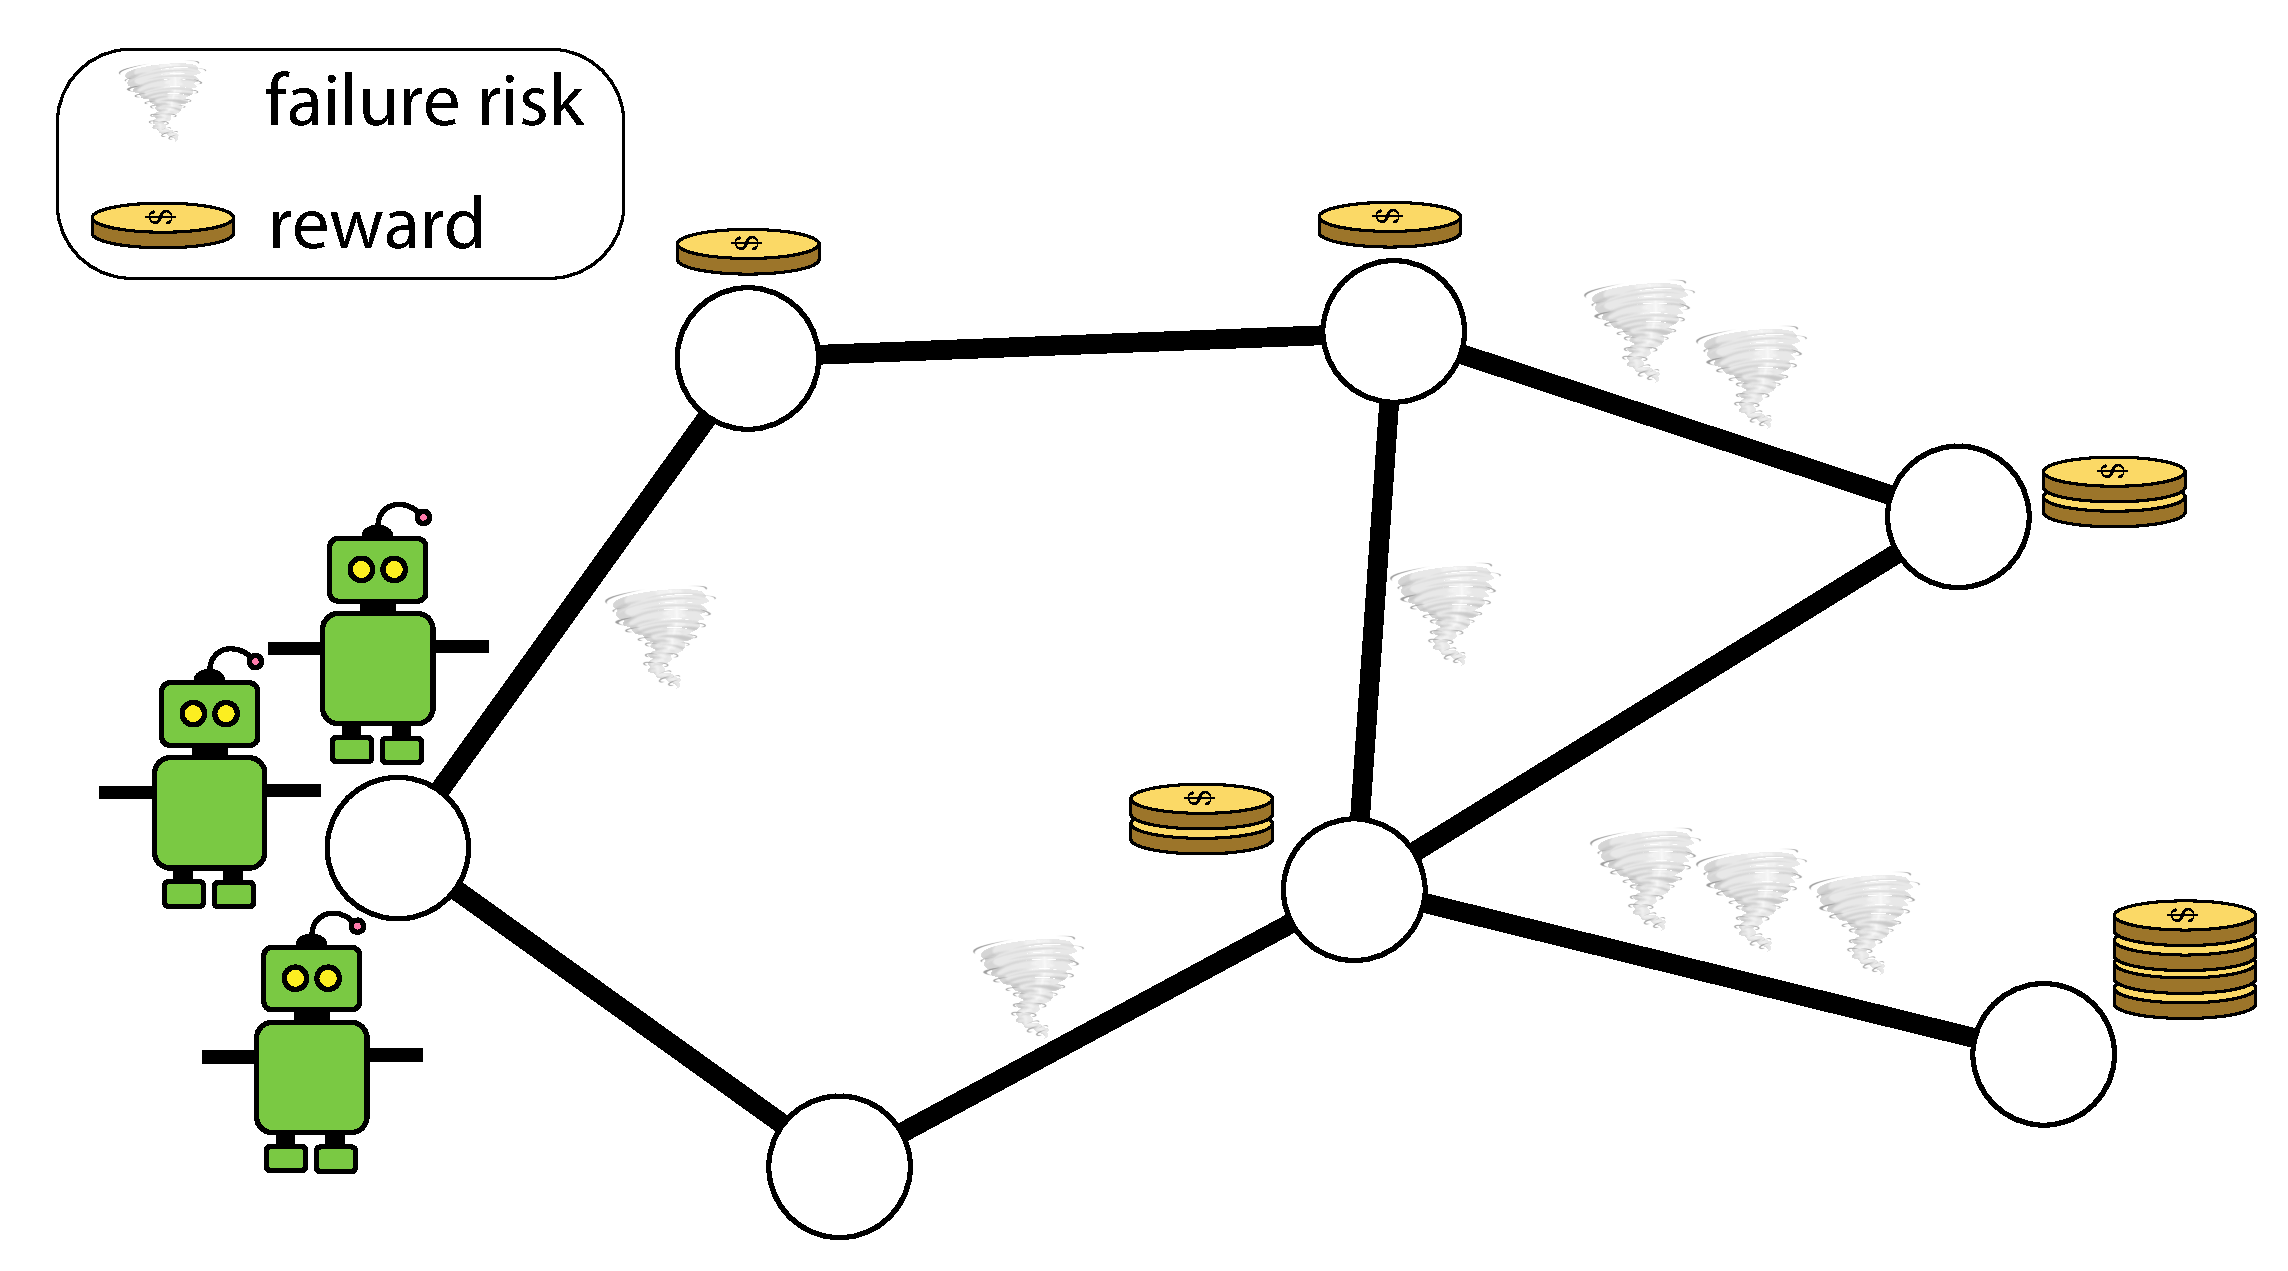
\includegraphics[width=0.6\textwidth]{overview.pdf}
    \caption{
       General problem setup. A team of robots are mobile on a graph. Each node of the graph offers a reward once visited by a robot. Each edge traversal by a robot imposes a risk of robot failure. Our utopian wish is for both a high collected team-reward and survival of the robots. {\color{red} show all possible paths and Pareto-plot? just two robots so easier.}
    }
    \label{fig:overview}
\end{figure}

The BO-RTOP follows the TSOP setup in Ref.~\cite{jorgensen2018team} but with three changes: we (i) omit the constraints that each robot survives above a threshold probability, (ii) allow robots to follow trails instead of paths (the latter prohibits a robot from visiting a node more than once), and (iii) aim to maximize two objectives instead of one.

\subsection{Problem setup}


\paragraph{Spatially abstracting the environment as a directed graph.}
We abstract the environment as a directed graph $G=(\mathcal{V}, \mathcal{E})$, where $\mathcal{V}$ is its set of vertices and $\mathcal{E}$ is its set of edges (ordered pairs of distinct vertices). We assume $G$ is strongly connected, but not necessarily complete.

\vspace{-\baselineskip}
\subparagraph{Interpretation.} 
Each node $v\in \mathcal{V}$ represents a distinct location in the environment (e.g., a room in a building or a house in a neighborhood).
Each edge $(v, v^\prime) \in \mathcal{E}$ represents a direct spatial connection for traveling from one location $v$ to another $v^\prime$ (e.g., a doorway or a road).


% the best (e.g., shortest or safest) path (in Euclidean space) for a mobile robot to take from the location represented by node $v$ to the location represented by $v^\prime$.
% Note, we do not assume the graph is complete\footnote{Ie., not every pair of distinct nodes $\{v, v^\prime\}$ is joined by two edges $(v, v^\prime)$ and $(v^\prime, v)$. 
% Eg., consider a building with node $v$ representing a room on the first floor, node $v^\prime$ a room on the second floor, and node $u$ as the staircase between the first and second floors. Traveling from node $v$ to node $v^\prime$ necessitates passing through node $u$ first.}.

\paragraph{The team of mobile robots.}
A homogenous team of $K$ robots all begin at a base station represented by node $v_b \in \mathcal{V}$ of the graph $G$. The robots are \emph{mobile} in the environment. I.e., generally, they may walk on the graph $G$.
% by travelling sequentially from one node $v$ to another node $v^\prime$ via traversing an edge $(v, v^\prime)\in\mathcal{E}$.

\paragraph{Team rewards offered by nodes in the graph.}
Each node $v\in \mathcal{V}$ in the graph $G$ offers rewards to the robot team, depending on the number of robots that visit it over the course of the mission. 
The node reward function $u_v: \mathbb{N}_{\geq 0} \rightarrow \mathbb{R}$ maps 
the number of robots that visit node $v$ over the course of the mission
% visits node $v$ receives by a robot over the course of the mission
 to 
 the additive reward accumulated by the team from node $v$.
Note, even if a robot fails after leaving node $v$, it still counts as a successful visit to node $v$.
In other words, the marginal reward offered by a node is immediately and irrevocably accumulated by the team after a robot visit.

\vspace{-\baselineskip}
\subparagraph{Interpretation.} The rewards given by a node represent the utility gained by the team when eg. robots deliver a unit of a resource to the node, take images of the node and transmit them back to the command center, actuate some process (eg. turn a valve) at the node, etc. 


\paragraph{The probabilistic model of robot failure/destruction during trail-following.} 
Each robot incurs a risk of failure/destruction when it traverses an edge of the graph $G$.
% following its trail $\rho$. 
Specifically, starting (in a functioning state) at some node $v$, a robot survives the two-step process of (i) traversing edge $(v, v^\prime) \in \mathcal{E}$ and (ii) visiting node $v^\prime$ with probability $\omega(v, v^\prime)$. 
We assume (i) each outcome (success or failure) of an edge traversal followed by a node visit by a robot is an independent event and (ii) survival probabilities are static over the course of the mission. 
Thus, from the function $\omega: \mathcal{E} \rightarrow (0, 1]$ that assigns robot survival probabilities to each edge of the graph $G$, we can compute the survival probabilities of the $K$ robots following any given set of walks.
% plans $\{\rho_1, ..., \rho_K\}$.% and (2) the expected utility of the rewards harvested by the robots along their paths, which we write next. 



\vspace{-\baselineskip}
\subparagraph{Interpretation.} The danger to a robot when traversing an edge could emanate from obstacles, rough terrain or seas, severe weather, mines, or adversaries capable of attacking the robots at the edge and/or sink node.
The survival/failure of a robot traversing an edge is stochastic owing to eg. (i) the unpredictable nature of an aerial robot crashing into an obstacle, a ground robot getting stuck in rocks/mud, or a surface aquatic robot succumbing to ocean waves or (ii) an adversary with imperfect detection and attack capabilities.

\vspace{-\baselineskip}
\subparagraph{Possible asymmetry.} We do not assume $\omega$ is symmetric, ie., that $\omega(v, v^\prime) = \omega(v^\prime, v)$. The traversal from node $v$ to $v^\prime$ may be more dangerous than from $v^\prime$ to $v$ owing to eg., (i, asymmetric edge traversal) strong air or water currents in the direction $v^\prime$ to $v$ or (ii, asymmetric dangers at nodes) an adversary with attack capability at node $v^\prime$ but not at $v$. %Even if edge traversal risks are symmetric, the action of visiting a node be risky, and node $v$ may be more or less dangerous than node $v^\prime$, breaking symmetry. 

\paragraph{The robot-team trail plans.}
To collect rewards, each robot on the team will plan to execute/follow a closed, directed trail $\rho$ on the graph $G$.  
The set of closed, directed trails $\mathcal{P}:=\{\rho_1, ..., \rho_K\}$ the robot-team plans to follow constitute the \emph{robot-team trail plans} for the \emph{mission}. These are only ``plans'' because a robot may fail in the process of following its planned trail and thus not actually visit all nodes in its trail plan.

\vspace{-\baselineskip}
\subparagraph{A closed, directed trail.} 
A \emph{directed trail} is an ordered list of nodes $\rho = (\rho[0], \rho[1], ..., \rho[\lvert \rho \rvert])$ where
(i) $\rho[i] \in \mathcal{V}$ is the $i$th node in the trail,  
(ii) $\lvert \rho \rvert$ is the number of edges traversed in the trail,
(iii) an edge exists from each node to the next node, ie., $(\rho[i-1], \rho[i])\in\mathcal{E}$ for $1 \leq i  \leq \lvert \rho \rvert$,
and 
(ii) the edges traversed in the trail are unique, ie. each edge in the multiset $\{(\rho[i-1], \rho[i])\}_{i=1}^{\lvert \rho \rvert}$ has a multiplicity of one.
Note, unlike a path, the nodes in a trail are not necessarily distinct \cite{wilson1979introduction}.
A \emph{closed} trail begins and ends at the same node, ie. $\rho [0]=\rho[\lvert \rho \rvert]$, which, here, $=v_b$.

\vspace{-\baselineskip}
\subparagraph{The static/offline setting.} 
The robot-team trail plan is set at the beginning of the mission, then followed by the robots without adaptation or updates during the mission (e.g., in reaction to realized robot failures). 
I.e., robots cannot communicate their status to the command center during the mission and/or the command center cannot send updated instructions to the robots after the mission executes.

\paragraph{Bi-objective, risky team orienteering problem.}
Given the graph $G$ as a spatial abstraction of the environment, the node reward functions $\{u_v : v \in\mathcal{V}\}$, the edge survival probability map $\omega$, and a homogenous team of $K$ mobile robots starting at the base node $v_b$, our goal in the \emph{bi-objective, risky team orienteering problem} is to determine the optimal robot-team [closed] trail plans $\{\rho_1, ..., \rho_K\}$ that maximize two-objectives, (1) the expected team-reward and (2) the expected number of robots that survive the mission:
\begin{equation}
\max_{\mathcal{P}=\{\rho_1, ..., \rho_K\}} [\mathbb{E}[U(\mathcal{P})], \mathbb{E}[R(\mathcal{P})]].
\label{eq:the_two_objs}
\end{equation}

\vspace{-\baselineskip}
\subparagraph{Objective \#1: the expected team reward collected by the robots.}
Let $T_v(\mathcal{P}) $ be the number of times node $v$ is visited by robots on a robot team with trail plans $\mathcal{P}$. Because of the stochastic nature of edge survival, and thus stochastic nature of which nodes the robots will survive to visit, $T_v$ is a random variable.
Then, the total team rewards collected by the robot-team following trail plan $\{\rho_1, ..., \rho_K\}$ is also a random variable:
\begin{equation}
U(\mathcal{P}) = \sum_{v\in\mathcal{V}} u_v\left ( T_v(\mathcal{P}) \right).
\end{equation}
We wish to maximize the expected team reward, $\mathbb{E}[U(\mathcal{P})]]$.

\vspace{-\baselineskip}
\subparagraph{Objective \#2: the expected number of robots that survive the mission.}
Let $R(\mathcal{P})$ be the number of robots, on a robot team with trail plans $\mathcal{P}$, that survive the mission. Because of the stochastic nature of edge survival, $R$ is a random variable. We wish to maximize the expected number of robots that survive the mission, $\mathbb{E}[R(\mathcal{P})] \in (0, K]$.

\subparagraph{Remarks on lacks of constraints/restrictions.} Note, we do not impose constraints on the survival probability of each individual robot as in the TSO formulation. We accept if one [unmanned] robot bears much more risk of destruction than another during the mission. Nor do we constrain the length of the planned trail of the robots. We assume each robot has sufficient fuel/electrical battery power to traverse the graph. We also do not assume the node reward function $u_v$ is necessarily submodular. E.g. in resource delivery, two deliveries could be required to construct some useful equipment from which utility is gained. {\color{red} right, then not diminishing returns?}
 It could be negative as well, if there is a penalty to visiting certain nodes.

\paragraph{Seeking the Pareto-optimal set of robot-team trail plans.} In most problem instances, there is a conflict between designing the robot-team trail plans that maximizing the expected reward vs. maximizing the number of robots that survive the mission. 
In one extreme, the robots safely stay at the base station and do not attempt to collect any rewards no matter the [positive] size of the rewards to be gained. 
At the other extreme, each robot plans to traverse the entire graph to attempt to collect each [suppose, positive and single-visit] reward no matter the risk.
In other words, there may not exist a utopian robot-team trail plan that simultaneously maximizes both objectives. 

{\color{red} here's where the simple example would help.}

Consequently, we seek

\subsection{Computing survival probabilities.}

\subsection{Computing expected reward.}
\paragraph{Survival probabilities.} 
We now derive some useful robot survival probabilities based on the risky-traversal model encoded in the robot survival probability function $\omega$.

\subparagraph{Survival of a robot following its trail.}
Let $S_n(\rho) : \{\text{fail}, \text{survive}\} \rightarrow \{0, 1\} $ be the Bernoulli random variable that is $1$ if a robot following trail $\rho$ survives to visit the $n$th node in this trail, and $0$ if it does not. For the event of survival, the robot must survive its traversal of \emph{all} of the first $n$ edges in its trail, so:
\begin{equation}
	\pi(S_n(\rho) = 1) = \prod_{i=1}^n \omega(\rho(i-1), \rho(i)) \text{ for } n\in \{1, ..., \lvert \rho \rvert\} \label{eq:pi_S_n}
\end{equation} The factorization owes to the independence of the edge-traversal$+$node-visit events.
The complement of the event of survival is failure, so $\pi(S_n(\rho) = 0)=1-\pi(S_n(\rho) = 1)$.

Of course, the outcome $S_n(\rho)=0$ implies $S_{n+i}(\rho)=0$ for $i \in \{1, ..., \lvert \rho \rvert - n\}$ since, once a robot fails along its trail, it cannot survive to visit nodes later in the trail.

\subparagraph{Survival of the team of robots following their trails.}
Let the random variable $R(\{\rho_1, ..., \rho_K\})$ be the number of robots that survive the mission, where the robot team follows trail plan $\{\rho_1, ..., \rho_K\}$. Owing to the independence of the edge-traversal events and thus of robot survival events, $R$ is the sum of the Bernoulli random variables giving the survival outcomes of each robot over its entire path:
\begin{equation}
	R(\{\rho_1, ..., \rho_K\})=\sum_{k=1}^K S_{\lvert \rho_k \rvert}(\rho_k). \label{eq:R_sum}
\end{equation}
Thus, $R$ follows the Poisson-Binomial distribution \cite{tang2023poisson}.
The probability that $r$ robots survive the mission is:
\begin{multline}
	\pi(R=r) = \sum_{\substack{\mathcal{R} \subseteq \{1, ..., K\}  \\ \lvert \mathcal{R} \rvert = r} } \,
	\prod_{k \in \mathcal{R}} \pi(S_{\lvert \rho_k \rvert}(\rho_k) = 1)
	\prod_{k \in \{1, ..., K\} \setminus \mathcal{R}} [1- \pi(S_{\lvert \rho_k \rvert}(\rho_k) = 1)], \\ \text{ for } r \in \{0, ..., K\}
	\label{eq:R_pb}
\end{multline} with $ \pi(S_{\lvert \rho_k \rvert}(\rho_k) = 1)$ in eqn.~\ref{eq:pi_S_n}.
Eqn.~\ref{eq:R_pb} sums over all $\binom{K}{r}$ possible size-$r$ surviving subsets $\mathcal{R}$ of the $K$ robots; the first product is the probability that all of those robots in $\mathcal{R}$ indeed survive their closed trails, and the second product is the probability that the other robots outside of $\mathcal{R}$ indeed fail somewhere along their closed trails.
Seen from eqn.~\ref{eq:R_sum}, the expected number of robots that survive the mission is:
\begin{equation}
	\mathbb{E}[R(\{\rho_1, ..., \rho_K\})]=\sum_{k=1}^K \mathbb{E}[S_{\lvert \rho_k \rvert}(\rho_k)] = \sum_{k=1}^K  \pi(S_{\lvert \rho_k \rvert}(\rho_k) = 1).
\end{equation}

\subparagraph{Visitation of a node by a robot following its trail.} 

{\color{red} theta I think is just the indices of the trail that correspond to node j. ordered list builder notation.}

\begin{equation}
	\theta_v(\rho) = (n : n \in (1, ..., \lvert \rho \rvert) ,  \rho(n) = v)
\end{equation}

Let the random variable $T_v(\rho)$ be the number of times a robot following trail $\rho$ visits node $v\in \mathcal{V} \setminus \{v_b\}$. 
% If node $v$ does not belong to the planned trail, of course, $T_v=0$. 
Equivalently, $T_v(\rho)$ is the number of edge-traversal events along the planned trail $\rho$ that (i) result in survival and (ii) land on node $v$ as the sink node. 
Thus, in terms of the robot-survival random variables $S_n(\rho)$:
\begin{equation}
	T_v(\rho) = \sum_{n \in \theta_v(\rho) } S_n(\rho), % \mathcal{I}[\rho(n) = v].
\end{equation}
where $\theta_v(\rho)$ is the strictly ordered set (list) of indices of the edges in the trail $\rho$ with sink node $v$:
\begin{equation}
	\theta_v(\rho) = (\{ n \in \{1, ..., \lvert \rho \rvert\} : \rho(n) = v\}, <).
\end{equation} So, $\lvert \theta_v(\rho) \rvert$ is the number of times node $v$ is planned to be visited by the robot following trail $\rho$, and successful traversal of the $\theta_v(\rho)(n)$th edge in the trail by the robot would be the $n$th time node $v$ is visited by that robot.
If node $v$ doesn't belong to the planned trail $\rho$ of the robot, the number of times node $v$ will be visited by the robot is zero with certainty ($T_v(\rho)=0$).
If node $v$ does belong to the trail $\rho$, the event that node $v$ is visited exactly $t$ times ($T_v(\rho)=t$) is equivalent to
(i) if $t=0$ (node $v$ is not visited), the event that the robot does not survive its first visit to node $v$, ie. $S_{\theta_v(\rho)(1)}=0$;
(ii) if $t=\lvert \theta_v(\rho)\rvert$ (node $v$ visitations equal to that in the plan), the event that the robot survives its last planned visit to node $v$, ie. $S_{\theta_v(\rho)(\lvert \theta_v(\rho) \rvert)}=1$;
(iii) if $1 \leq t < \lvert \theta_v(\rho ) \rvert$, the event that (a) the robot survives its $t$th planned visit to node $v$ and (b) does not survive its $(t+1)$th planned visit, ie. $(S_{\theta_v(\rho)(t)}=1) \land (S_{\theta_v(\rho)(t+1)}=0)$. So, the probability mass function of $T_v(\rho)$ is:
\begin{equation}
	\pi(T_v(\rho) = t ) = 
	\begin{cases}
		\begin{cases}
			1, & t = 0 \\
			0, & 1 \leq t \leq \lvert \theta_v(\rho ) \rvert  \\
		\end{cases}
		&  v \notin \rho \\
		\begin{cases}
			\pi(S_{\theta_v(\rho)(1)}=0), & t = 0 \\
			\pi\left( (S_{\theta_v(\rho)(t)}=1) \land (S_{\theta_v(\rho)(t+1)}=0)\right), &1 \leq t < \lvert \theta_v(\rho ) \rvert   \\
			\pi\left( (S_{\theta_v(\rho)(\lvert \theta_v(\rho) \rvert)}=1) \right), & t = \lvert \theta_v(\rho ) \rvert   \\
			0 , & t >  \lvert \theta_v(\rho ) \rvert
		\end{cases}
		& v \in \rho
	\end{cases}
\end{equation}
with
\begin{align}
\pi\left( (S_{\theta_v(\rho)(t)}=1) \land (S_{\theta_v(\rho)(t+1)}=0)\right) &=
\pi\left( S_{\theta_v(\rho)(t+1)}=0 \mid S_{\theta_v(\rho)(t)}=1)\right)
\pi (S_{\theta_v(\rho)(t)}=1) \\
&= \left(1-\prod_{i=\theta(t)+1}^{\theta(t+1)} \omega(\rho(i-1), \rho(i)) \right) \prod_{i=1}^{\theta(t)} \omega(\rho(i-1), \rho(i)).
\end{align}

\subparagraph{Visitation of a node by the team of robots following their trails.} 
The number of times node $v$ is visited by \emph{any} robot belonging to the robot team following trail plan $\{\rho_1, ..., \rho_K\}$ is
\begin{equation}
	T_v(\{\rho_1, ..., \rho_K\} ) = \sum_{k=1}^K T_v(\rho_k),
\end{equation} owing to independence of the robot survival events. 
Its probability mass function sums over all possible ways to split the $t$ visits of node $v$ among the $K$ robots:
\begin{equation}
	\pi(T_v(\{\rho_1, ..., \rho_K\} = t) = 
	% \sum_{t_1 \in \{0, ..., \lvert \theta_v(\rho_1) \rvert\} } \cdots  \sum_{t_K \in \{0, ..., \lvert \theta_v(\rho_K) \rvert\} } 
	\sum_{t_1 + \cdots t_K = t}
	\prod_{k=1}^K \pi(T_v(\rho_k)=t_k),
\end{equation} with $t_k \in \{ 0, ..., \lvert \theta_v(\rho_k) \rvert\} $ the number of times robot $k$ visits node $v$.

% The number of robots on the team, with trail plans $\{\rho_1,...,\rho_K\}$, that visit node $v$ is $\sum_{k=1}^K Z_v(\rho_k)$.
% HUGE MESS: if trails not paths, then can visit a node more than once. think of a star graph. then this is not a sum of independent variables.


\subsection{Total utility gained by the robot-team from node-visits}
Finally, the reason the robots are following their trails on the graph is to collect rewards from the nodes.
Each node $v\in \mathcal{V}$ in the graph $G$ offers rewards to the team if visited by robot(s) on the team. 
Let $u_v: \mathbb{N}_{\geq 0} \rightarrow \mathbb{R}_{\geq 0}$ be a utility function that maps 
the number of visits node $v$ receives by a robot over the course of the mission
 to 
 the additive reward accumulated by the team from that node.
Note, even if the robot fails after leaving a node, it counts as a visit to that node.
In other words, the reward offered by a node is immediately and irrevocably accumulated by the team after a visit by a robot on the team.
Then, the total utility collected by the robot-team following trail plan $\{\rho_1, ..., \rho_K\}$ is the random variable:
\begin{equation}
U(\{\rho_1,...,\rho_K\}) = \sum_{v\in\mathcal{V}\setminus \{v_b\}} u_v\left ( T_v(\{\rho_1, ..., \rho_K\}) \right).
\end{equation}
(The base node $v_b$ does not offer reward to the team.)

The expectation utility accumulated over the mission by a robot-team following trail plan $\{\rho_1, ..., \rho_K\}$ is:
\begin{equation}
	\mathbb{E}[U(\{\rho_1,...,\rho_K\})]= \sum_{v\in\mathcal{V}\setminus \{v_b\}} \sum_{t= 0}^{\sum_{k=1}^K \lvert \theta_v(\rho_k) \rvert } t u_v(t) \pi(T_v(\{\rho_1, ..., \rho_K\}) = t)
\end{equation}
% I can handle non-diminishing returns! e.g. if two visits better than one.

\subparagraph{Single-visit rewards.}
In the case of single-visit rewards, a node can offer reward to only a single robot. I.e., once a node is visited, it does not offer further rewards to the team. Then, the utility function is
\begin{equation}
	u_v(k) = \begin{cases}
		0 & k = 0 \\
		\upsilon_v & k \geq 1,
	\end{cases}
\end{equation} where $\upsilon_v \in \mathbb{R}_{\geq 0}$ is the reward offered by node $v$. And, the expected team-reward is:
\begin{align}
	\mathbb{E}[U(\{\rho_1, ..., \rho_K\}) & = \sum_{v \in \mathcal{V} \setminus \{v_b\}} \upsilon_v \pi(T_v(\{\rho_1, .., \rho_K\}) \geq 1) \\
		      & = \sum_{v \in \mathcal{V} \setminus \{v_b\}} \upsilon_v \left(1 - \prod_{k=1}^K  \pi(T_v(\rho_k) =0) \right)
\end{align} since the event that node $v$ is visited by one or more robots is the complement of the event that none of the robots on the team visit it.

\subparagraph{Multi-visit rewards.}

\subsection{The bi-objective optimization problem}


There may not exist a utopian robot-team trail plan that simultaneously maximizes both objectives. 
That is, these two objectives may compete, implying the ultimate team trail plan selected for the mission may depend on a tradeoff between the expected utility and the expected survival; making this tradeoff requires invoking values held by a (human) decision-maker. Intuitively, valuing survival more than utility will favor trail-plans where robots do not enter dangerous regions of the environment, even if large rewards are contained there, and valuing utility more than survival will instead send robots into these dangerous regions to attempt collection of those rewards. 

Owing to the inherent tradeoff between survivability and collected reward, herein we seek the Pareto-optimal set of team-robot trail plans. Then, we present the Pareto set to the decision-maker, who ultimately selects the team-robot trail-plans according to his or her values in terms of the importance of team-reward vs. robot survival. 

\paragraph{Pareto-optimal team-robot trail plans.} 
A Pareto-optimal robot-team trail plan $\mathcal{P}:\{\rho_1, ..., \rho_K\}$ cannot be altered to
(1) increase the survivability objective $E[R(\mathcal{P})]$ without compromising (decreasing) the utility objective $E[U(\mathcal{P})]$
nor
(2) increase the utility objective $E[U(\mathcal{P})]$ without compromising (decreasing) the survivability objective $E[R(\mathcal{P})]$.
Formally, a team trail plan $\mathcal{P}:=\{\rho_1, ..., \rho_K\}$ Pareto-dominates team trail plan  $\mathcal{P}^\prime :=\{\rho_1^\prime, ..., \rho_K^\prime\}$ if both
\begin{align}
	\mathbb{E}[U(\mathcal{P})] \geq \mathbb{E}[U(\mathcal{P}^\prime)] & \text{ and }  \mathbb{E}[R(\mathcal{P})] \geq \mathbb{E}[R(\mathcal{P}^\prime)] \\
	\mathbb{E}[U(\mathcal{P})] > \mathbb{E}[U(\mathcal{P}^\prime)] & \; \text{ or   } \; \mathbb{E}[R(\mathcal{P})] > \mathbb{E}[R(\mathcal{P}^\prime)].
\end{align}
A plan $\mathcal{P}$ belongs to the Pareto-optimal set of plans if no other trail plan $\mathcal{P}^\prime$ Pareto-dominates it.


% harvest risk different from visit risk. once harvested, then no longer risk for other robots to visit that node.

\section{Bi-objective ant colony optimization}
To find the [approximate] set of Pareto-optimal robot-team trail plans, with respect to the two objectives in eqn.~\ref{eq:the_two_objs}, we resort to bi-objective (BO) ant colony optimization (ACO) \cite{iredi2001bi}. 
ACO \cite{dorigo2006ant}, a form of swarm intelligence \cite{bonabeau1999swarm} inspired by ants foraging for food via pheromone trails \cite{bonabeau2000inspiration}, is a meta-heuristic for combinatorial optimization problems---particularly naturally-suited for finding optimal paths on graphs. 

% stigmergy
We have a colony of $N_{\text{ants}}$ artificial ants that search for Pareto-optimal team-robot trail plans. 
ACO proceeds in iterations. 
At each iteration, each ant in the colony constructs a robot-team trail plan $\{\rho_1, ..., \rho_K\}$. 
The ants collaborate in the search, in that they maintain a shared, global set of Pareto-optimal team-robot trail plans.

The ant colony is heterogeneous; each ant is assigned a parameter $\lambda \in [0, 1]$ that dictates how it will balance the two objectives as it searches for a Pareto-optimal team-robot trail plan. Particularly, ant $i\in\{1, ..., N_{\text{ants}}\}$ in the colony is assigned $\lambda_i := (i-1) / (N_{\text{ants}}-1)$. A $\lambda$ closer to zero (one) implies the ant prioritizes maximizing the expected utility $E[U]$ (expected survivability $E[R]$). The idea of having a heterogeneous colony is that each ant focuses on finding robot-team trail-plans belonging to different regions of the Pareto front. 

Each ant constructs a team-robot trail plan $\{\rho_1, ..., \rho_K\}$ sequentially, robot-by-robot; i.e., the ant fully constructs the closed trail for robot 1, $\rho_1$, then $\rho_2$, and so on. And, the construction of a trail by an ant proceeds node-by-node, starting at the base node $v_b$; i.e., the ant follows the trail the robot plans to take. Suppose the ant is constructing the closed trail for robot $k$, $\rho_k$, and currently sits at node $x=\rho_k(i)$, meaning that the ant has chosen the first $i$ nodes of robot $k$'s trail, with the partial trail being $\rho_k^\dagger=(v_b, \rho_k(1), ..., \rho_k(i))$. 
The next node $y=\rho_k(i+1)$ in the trail is chosen probabilistically among those viable, with probability defined according to (i) the amounts $\tau_u(x, y)$ and $\tau_r(x, y)$ of two species of pheromone on the edge from $x$ to $y$ that pertain to the ants' past experience of traversing this edge with respect to the $\mathbb{E}[U]$ and $\mathbb{E}[R]$ objective, (ii) our heuristics $\eta_u(x, y)$ and $\eta_r(x, y)$  that define the [greedy] appeal of taking the edge $u$ to $v$ with goals of optimizing the $\mathbb{E}[U]$ and $\mathbb{E}[R]$ objective, (iii) the previously constructed robot trails $\{\rho_1, ..., \rho_{k-1}\}$, and (iv) how the ant balances the two objectives, encoded in its $\lambda$:
\begin{equation}
	\pi(y \mid x) = 
	\begin{cases}
		\dfrac{
		 \left[\tau_r(x, y) \eta_r(x, y) \right]^\lambda \left[ \tau_u(x, y) \eta_u(x, y; \{\rho_1, ..., \rho_{k-1}\}) \right]^{1-\lambda} }{
		 \sum_{y^\prime \in \mathcal{V}^\dagger} \left[\tau_r(x, y^\prime) \eta_r(x, y^\prime) \right]^\lambda \left[ \tau_u(x, y^\prime) \eta_u(x, y^\prime; \{\rho_1, ..., \rho_{k-1}\}) \right]^{1-\lambda} 
		 }
		 &
		 y \in \mathcal{V}^\dagger
		  \\
		 0, & y \notin \mathcal{V}^\dagger
	\end{cases} \label{eq:prob_x_y}
\end{equation} where the set of viable next-nodes in the trail, $y=\rho(i+1)$, are those serving as a sink node for an edge (i) whose source node is $x=\rho(i)$ and (ii) has not already been taken in the partial trail $\rho_k^\dagger$:
\begin{equation}
 	\mathcal{V}^\dagger := \{ y : (x, y) \in \mathcal{E} \land \nexists j \in \{1, ..., i\} : (\rho_k^\dagger(j), \rho_k^\dagger(j+1))= (x, y)  \}.
\end{equation}
We next explain the pheromone and the heuristic.

\paragraph{Pheromone.} The ants lay two distinct species of artificial pheromone on the edges of the graph $G$---one species for each objective. Let the functions $\tau_r:\mathcal{E}\rightarrow \mathbb{R}_+$ ($\tau_u:\mathcal{E}\rightarrow \mathbb{R}_+$) give the amount of the pheromone species on the edges of the graph $G$ that represent their promise, learned from the past experience of ants, for belonging to robot trails that maximize the expected number of robots that survive $\mathbb{E}[R]$ (the expected team utility gained by the robots $\mathbb{E}[U]$). Thus, when selecting the next node for a trail, eqn.~\ref{eq:prob_x_y} specifies that ants are more likely to traverse an edge if it has a large amount of pheromone on it; depending on the ant's value of $\lambda$, its decision places more or less emphasis on $\tau_u$ vs. $\tau_r$. Note, the pheromone functions are not static, but change from iteration-to-iteration. 


\paragraph{Heuristic.}

\begin{align}
\eta_r(x, y) & := \omega(x, y) \\
\eta_u(x, y, \{\rho_1, ..., \rho_{k-1}\}) & :=  \omega(x, y) \mathbb{E}[u_v(T_v(\{\rho_1, ..., \rho_{k-1}\})+1)]
\end{align}
marginal expected reward


\paragraph{Laying pheromone.}

\section{Results}

\paragraph{DARPA power plant}

Defense Advanced Research Projects Agency (DARPA) Subterranean (SubT) Challenge \cite{chung2023into}


\section{Discussion}

Much future work remains.
The risky orienteering problem can be extended to account for more real-world complexity, such as (a) fuel/battery constraints for the robots and perhaps nodes that serve as fuel/recharging stations, (b) stochastic rewards.


analytical case? star graph.

other risk metrics \cite{majumdar2020should}.

non-independent edge hops. eg. adversary in certain area, or not.

Future work. online.

if observed then reward diminished.


\bibliography{refs}
\bibliographystyle{unsrt}

\end{document}  
